\subsection{Eure Profs}
Um euch einen kleinen Vorgeschmack auf die Leute zu geben, die euch demn"achst mit ihrem Wissen begl"ucken wollen, seien sie hier kurz aufgef"uhrt:
\subsubsection{Algorithmen und Datenstrukturen}

\begin{figure}[h]
	\centering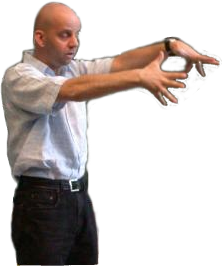
\includegraphics[width=0.7\linewidth]{bilder/dozenten/fekete_frei.png}\\
	{Prof. S\'andor Fekete}
\end{figure}
Diese Vorlesung vermittelt Programmiersprachenunabh"angige Konzepte wie B"aume, Listen oder Stacks. Wer nicht wei"s, was sich hinter diesen Begriffen verbirgt, sollte auf keinen Fall die "Ubungen verpassen.

\begin{figure}[h]
	\centering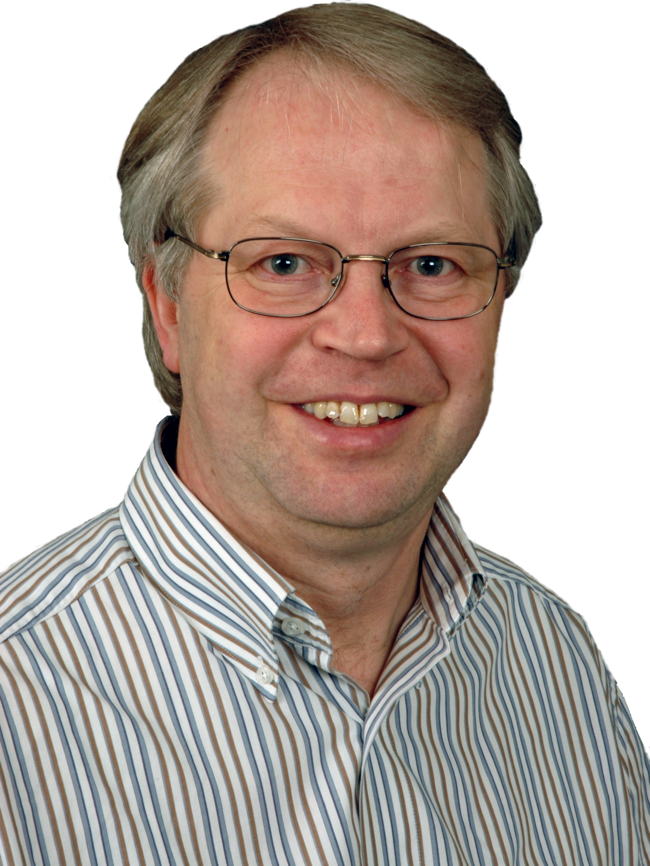
\includegraphics[width=0.6\linewidth]{bilder/dozenten/struck.png}\\
	{Dr. Werner Struckmann}
\end{figure}
\subsubsection{Programmieren 1}

Programmiert wird hier fast ausschlie"slich in Java. Wer keine oder nur wenig Erfahrungen mit Java gemacht hat, sollte unbedingt die kleinen "Ubungen bearbeiten.
%Die Klausur ist ber"uhmt f"ur ihre hohe Durchfallquote! (Gl"ucklicherweise sind daran nicht die Informatiker schuld)
%Trotzdem: Programmieren ist das Handwerk der Informatik, also macht eurem Fach Ehre.

\subsubsection{Lineare Algebra}

\begin{figure}[h]
	\centering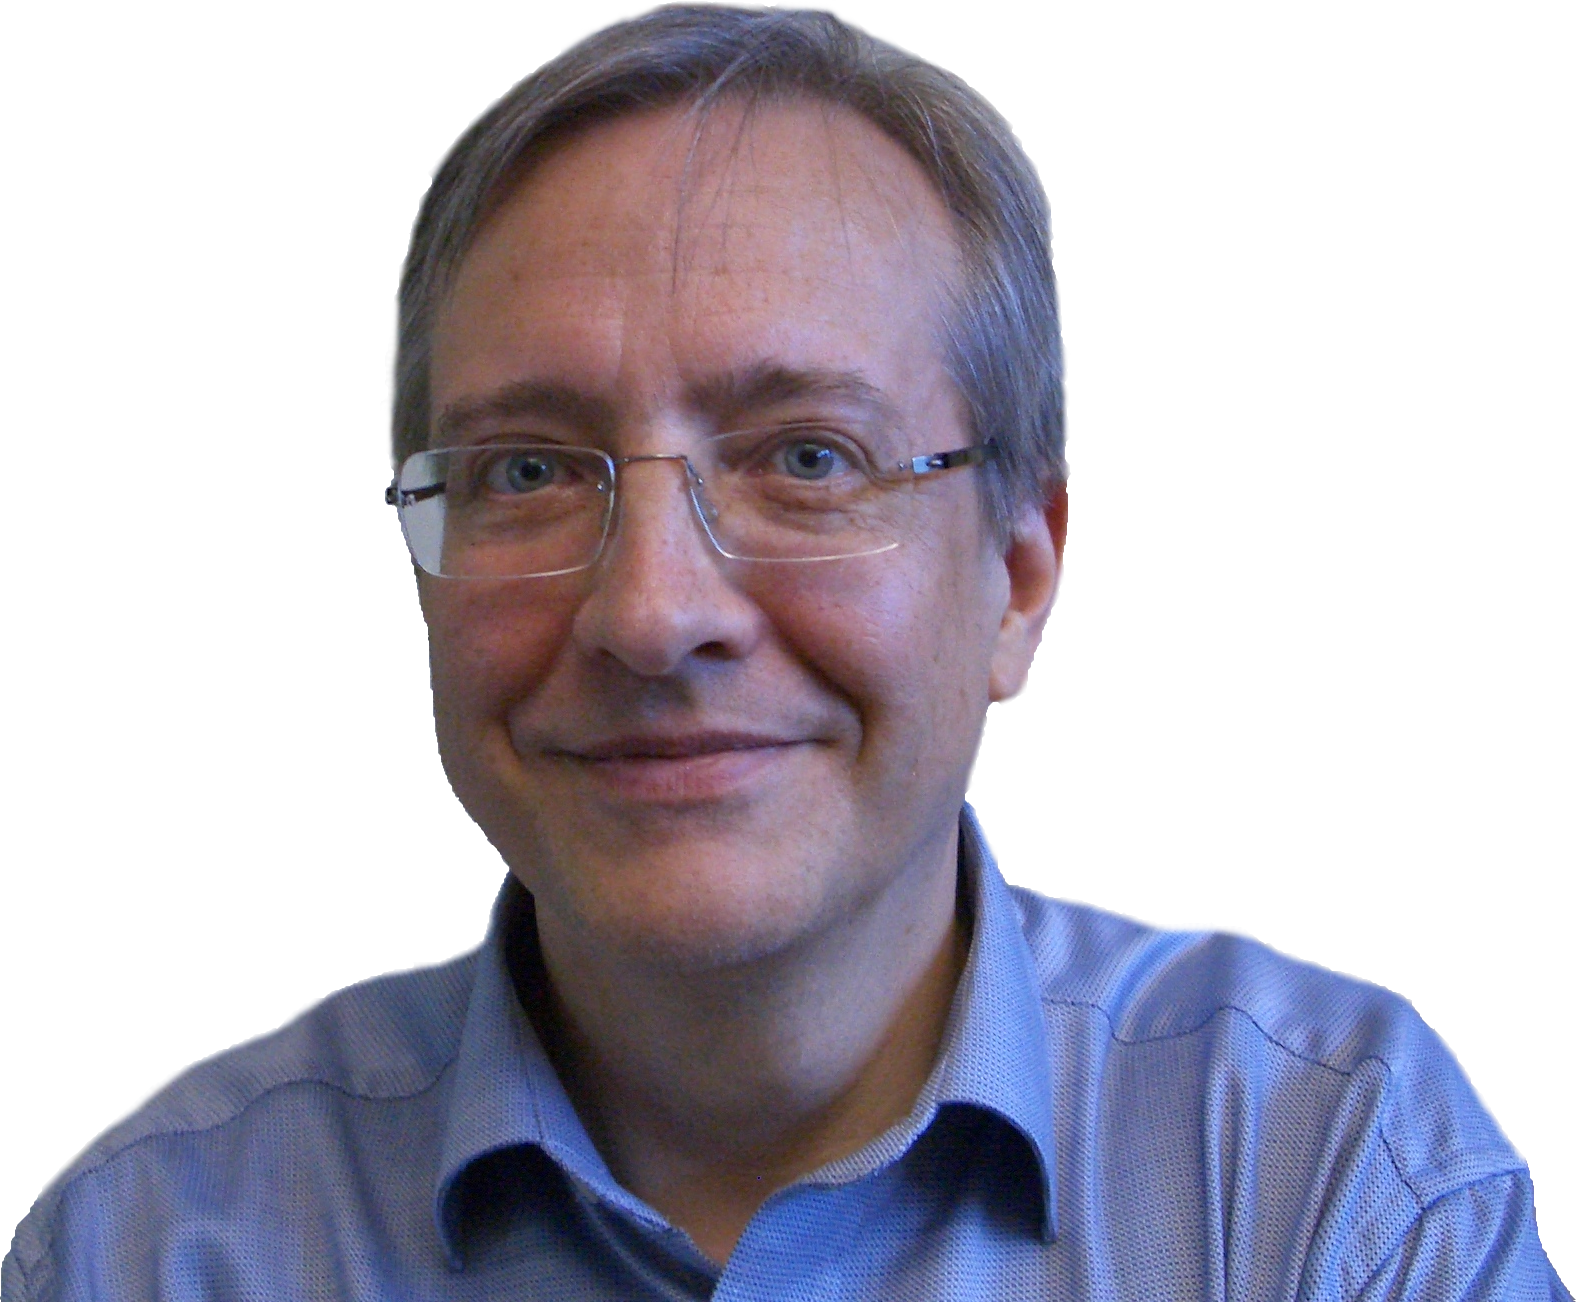
\includegraphics[width=0.8\linewidth]{bilder/dozenten/marten_frei.png}\\
	{Dr. Wolfgang Marten}
\end{figure}
Hier geht es um Vektoren und Matrizen, sowie ein wenig Gruppentheorie.
Die "Ubungen sind zwar nicht immer einfach, geben aber einen sehr guten Ausblick auf die Klausur.

\subsubsection{Diskrete Mathematik}

% \begin{figure}[h]
% 	\centering\includegraphics[width=0.7\linewidth]{bilder/kemnitz.png}\\
% 	{Dr. Arnfried Kemnitz}
% \end{figure}
Diskrete Mathematik handelt von allem, was mit ganzen Zahlen zu tun hat: Fibbonacci-Zahlen, Primzahlen, Modulorechnung, usw.
Die Veranstaltung wird von Dr. Arnfried Kemnitz gehalten (leider kein Foto).

\begin{figure}[h]
  \centering
  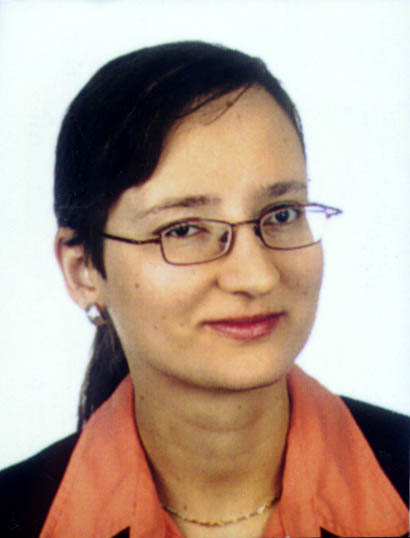
\includegraphics[width=0.7\linewidth]{bilder/dozenten/Andrea.jpg}\\
  {Dr. Andrea Herrmann}
\end{figure}
\subsubsection{Wissenschaftliches Arbeiten}

\begin{figure}[h]
	\centering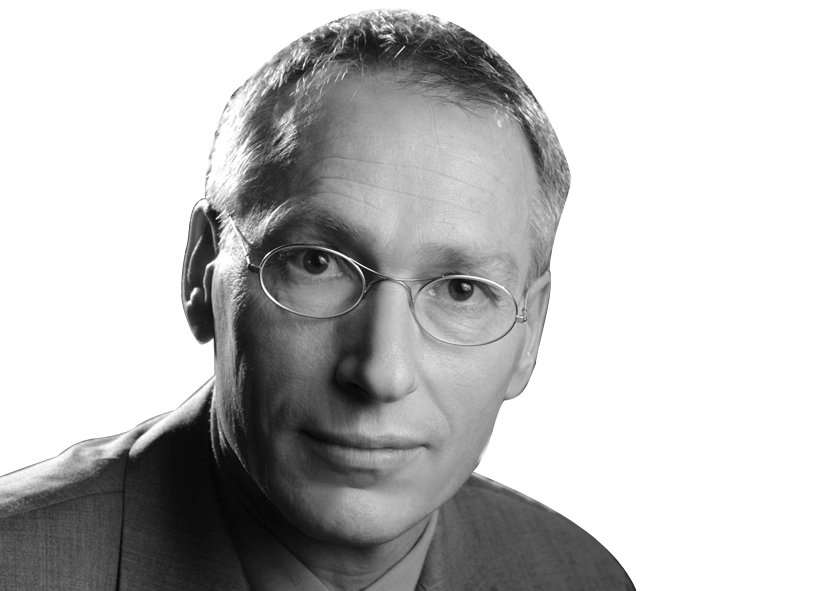
\includegraphics[width=0.9\linewidth]{bilder/dozenten/jung_frei.png}\\
	{Prof. Helmut Jung}
\end{figure}
In dem Kurs "`wissenschaftliches Arbeiten"' lernen die Teilnehmer/-innen, Schritt f"ur Schritt eine wissenschaftliche Arbeit durchzuf"uhren -- beispielsweise eine Bachelorarbeit.
Hierzu erfahrt ihr, wie man systematisch vorgeht und welche Methoden man in welchem Schritt verwenden kann.
Die Veranstaltung findet in zwei Gruppen statt, eine bei Prof. Jung und die andere bei Dr. Herrmann.
% Das gehört eigentlich nicht hier hin:

%Die Veranstaltung wird in zwei Gruppen angeboten: Der erste Kurs bei Prof. Jung findet Montag von 9:45 bis 11:15 Uhr und Dienstag von 11:30 bis 14:45 Uhr statt.
%Der zweite Kurs bei Dr. Herrmann findet Dienstag von 15:00 bis 16:30 Uhr statt.
%Beide Kurs haben denselben Inhalt und dieselbe Stundenzahl.
%Der zweite Kurs dauert das gesamte Semester, der andere endet entsprechend fr"uher.
